\documentclass[conference]{IEEEtran}
\IEEEoverridecommandlockouts
% The preceding line is only needed to identify funding in the first footnote. If that is unneeded, please comment it out.
%Template version as of 6/27/2024

\usepackage{cite}
\usepackage{amsmath,amssymb,amsfonts}
\usepackage{algorithmic}
\usepackage{graphicx}
\usepackage{textcomp}
\usepackage{xcolor}

\def\BibTeX{{\rm B\kern-.05em{\sc i\kern-.025em b}\kern-.08em
    T\kern-.1667em\lower.7ex\hbox{E}\kern-.125emX}}
\begin{document}


\title{Conference Paper Title*\\
{\footnotesize \textsuperscript{*}Note: Sub-titles are not captured for https://ieeexplore.ieee.org  and
should not be used}
\thanks{Identify applicable funding agency here. If none, delete this.}
}

\author{\IEEEauthorblockN{Jos\`e Dalla Torre}
\IEEEauthorblockA{\textit{Machine Learning and Perception Lab} \\
\textit{University of Udine}\\
Udine, Italy \\
dallatorre.josezito@spes.uniud.it}
\and
\IEEEauthorblockN{Christian Micheloni}
\IEEEauthorblockA{\textit{Machine Learning and Perception Lab} \\
\textit{University of Udine}\\
Udine, Italy \\
christian.micheloni@uniud.it}
\and
\IEEEauthorblockN{Gian Luca Foresti}
\IEEEauthorblockA{\textit{Machine Learning and Perception Lab} \\
\textit{University of Udine}\\
Udine, Italy \\
gianluca.foresti@uniud.it}
}

\maketitle

\begin{abstract}
This document is a model and instructions for \LaTeX.
This and the IEEEtran.cls file define the components of your paper [title, text, heads, etc.]. *CRITICAL: Do Not Use Symbols, Special Characters, Footnotes, 
or Math in Paper Title or Abstract.
\end{abstract}

\begin{IEEEkeywords}
component, formatting, style, styling, insert.
\end{IEEEkeywords}

\section{Introduction}
This document is a model and instructions for \LaTeX.
Please observe the conference page limits. For more information about how to become an IEEE Conference author or how to write your paper, please visit   IEEE Conference Author Center website: https://conferences.ieeeauthorcenter.ieee.org/.

\subsection{Maintaining the Integrity of the Specifications}
Test citation \cite{IEEEexample:bluebookstandard}

\section{ball action spotting challenge}
ball action spotting challenge
 ball action spotting, focusing on retrieving all
timestamps related to the soccer ball change of
state,

\section{The dataset}
The dataset is \cite{Deliège2020SoccerNetv2}

\section{First solution with paper}
I need to cite the paper and describe it

\section{Second solution I based my solution on}
Second solution I based my solution on
\section{My solution}
My solution

\subsection{\LaTeX-Specific Advice}

``Fig.~\ref{fig}'', even at the beginning of a sentence.

\begin{table}[htbp]
\caption{Table Type Styles}
\begin{center}
\begin{tabular}{|c|c|c|c|}
\hline
\textbf{Table}&\multicolumn{3}{|c|}{\textbf{Table Column Head}} \\
\cline{2-4} 
\textbf{Head} & \textbf{\textit{Table column subhead}}& \textbf{\textit{Subhead}}& \textbf{\textit{Subhead}} \\
\hline
copy& More table copy$^{\mathrm{a}}$& &  \\
\hline
\multicolumn{4}{l}{$^{\mathrm{a}}$Sample of a Table footnote.}
\end{tabular}
\label{tab1}
\end{center}
\end{table}

\begin{figure}[htbp]
\centerline{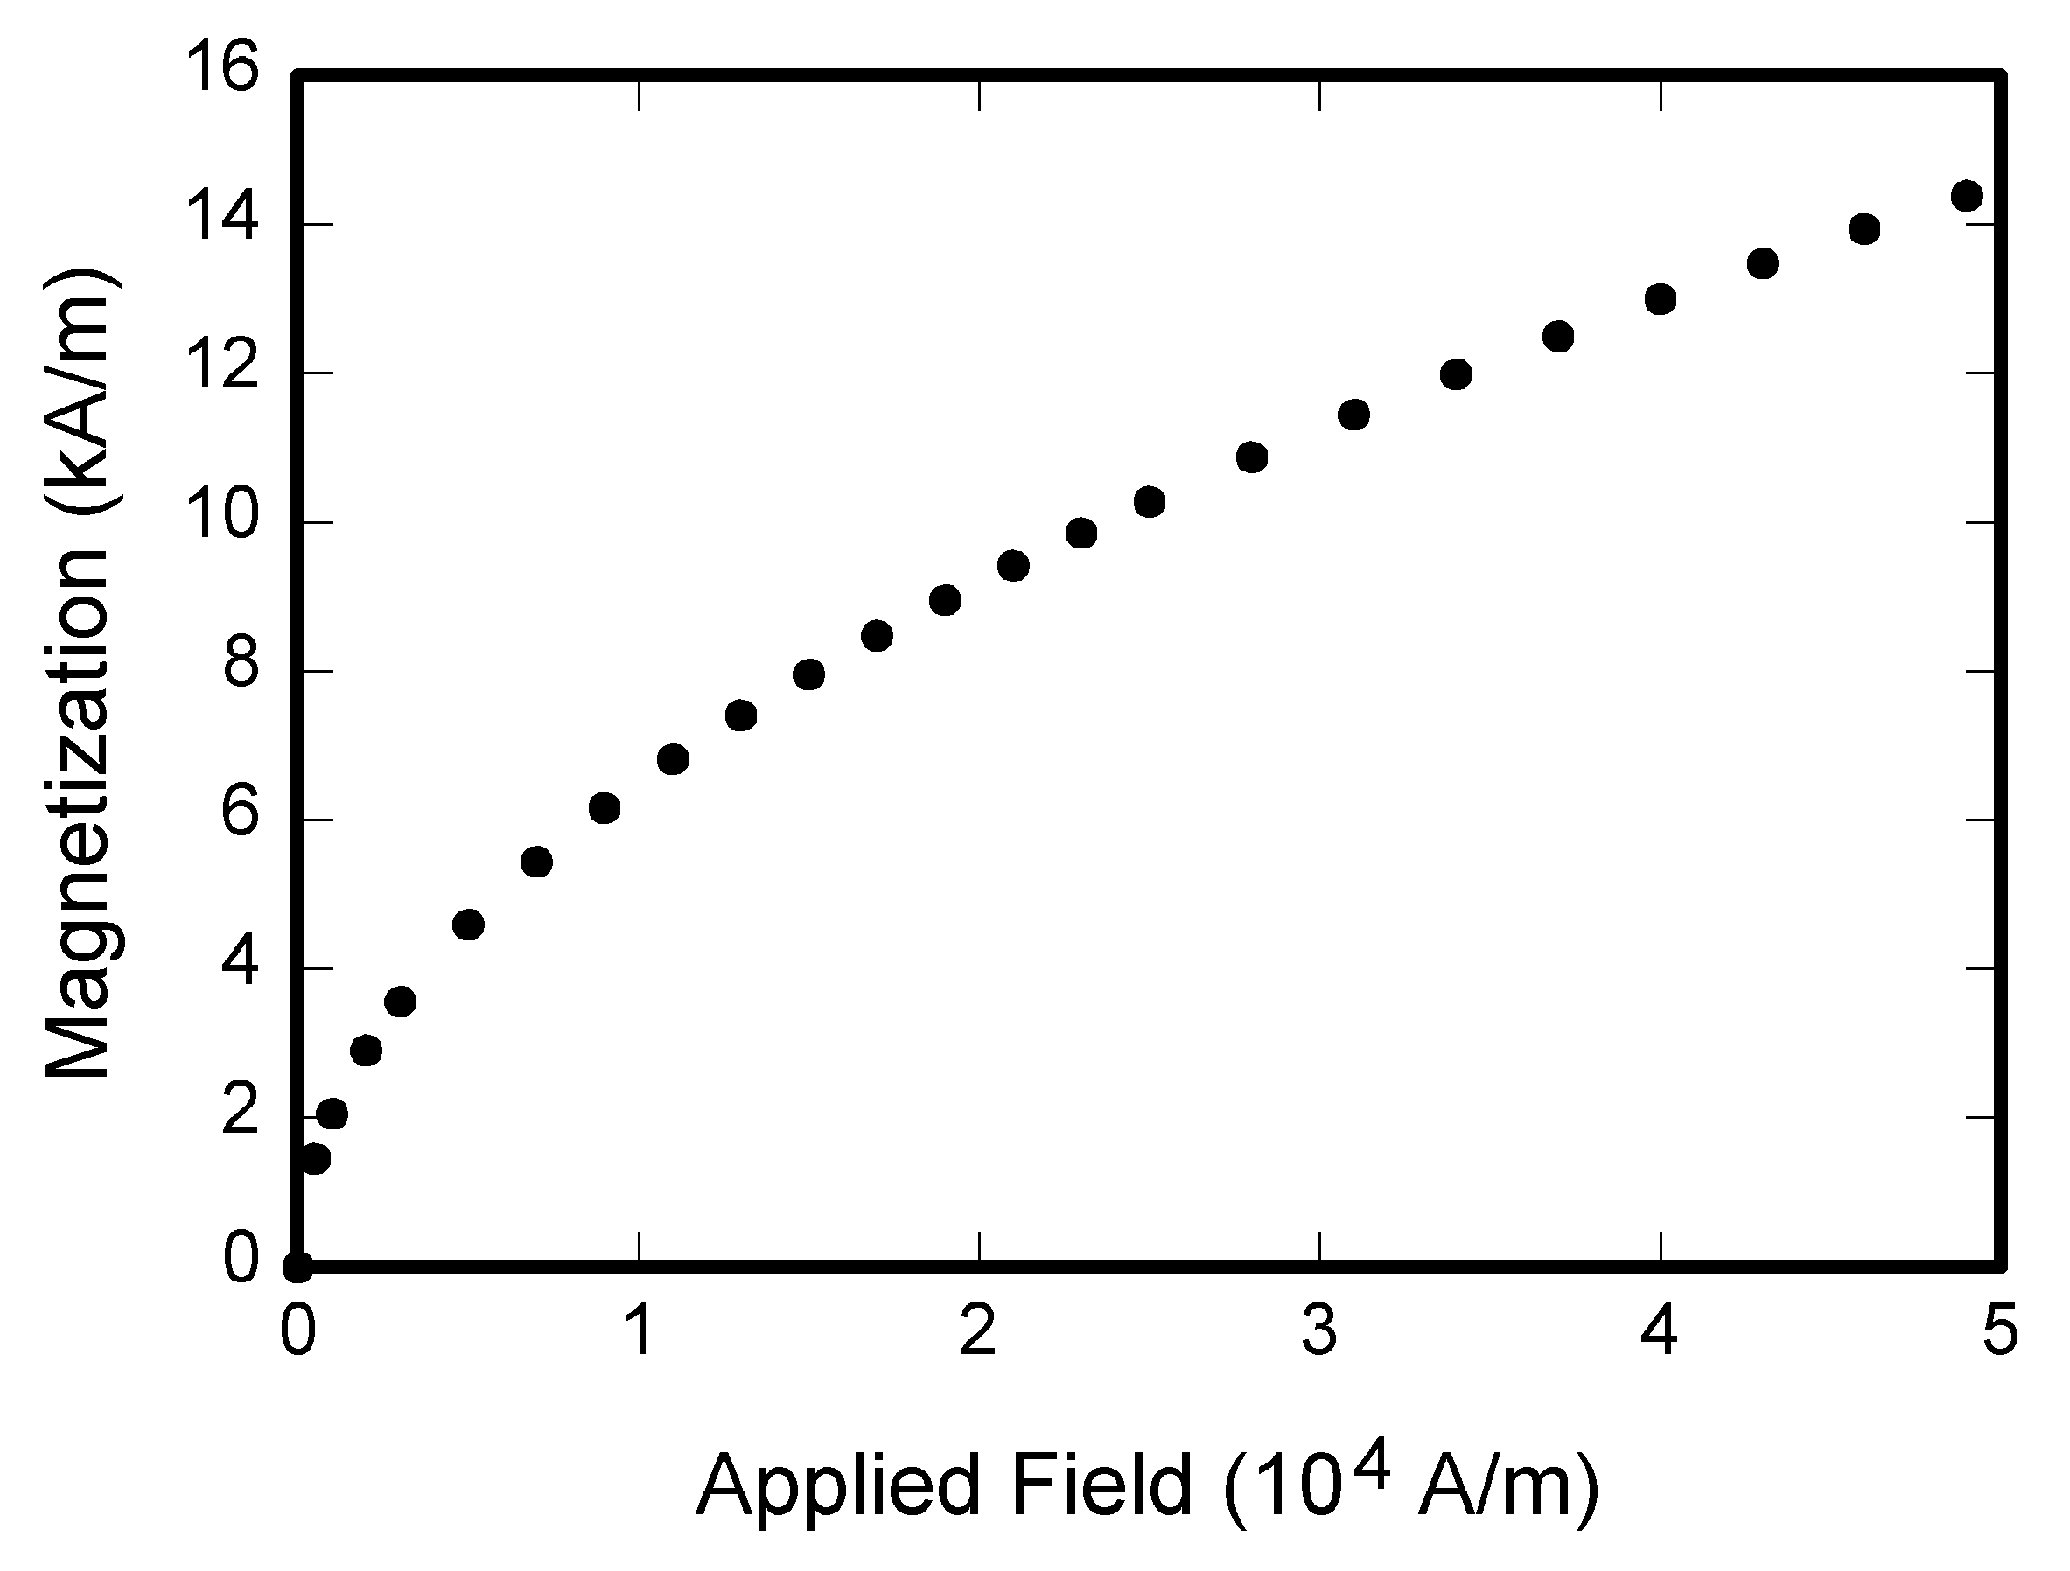
\includegraphics{fig1.png}}
\caption{Example of a figure caption.}
\label{fig}
\end{figure}


\section*{Acknowledgment}

\section*{References}

\bibliography{IEEEabrv.bib,IEEEexample.bib}{}
\bibliographystyle{IEEEtran}

\vspace{12pt}
\color{red}
IEEE conference templates contain guidance text for composing and formatting conference papers. Please ensure that all template text is removed from your conference paper prior to submission to the conference. Failure to remove the template text from your paper may result in your paper not being published.

\end{document}
